\documentclass[fleqn]{article}
\usepackage{graphicx}
\usepackage{amsmath,amsfonts,amssymb}
\usepackage{commath}

\usepackage{titlesec}
\titlelabel{\thetitle)\quad}

\usepackage{changepage,titlesec}
\titleformat{\section}[block]{\bfseries}{\thesection)}{1em}{}
\titleformat{\subsection}[block]{}{(\thesubsection)}{1em}{}
\titleformat{\subsubsection}[block]{}{(\thesubsubsection)}{1em}{}
\titlespacing*{\subsection} {2em}{3.25ex plus 1ex minus .2ex}{1.5ex plus .2ex}
\titlespacing*{\subsubsection} {4em}{3.25ex plus 1ex minus .2ex}{1.5ex plus .2ex}

\usepackage{geometry}
\geometry{
	a4paper,
	total={170mm,257mm},
	left=20mm,
	top=20mm,
}

\title{Homework 9}
\author{Submitted By: Puneet Singhal\\}
\date{}

\def\thesubsection{\alph{subsection}}
\def\thesubsubsection{\roman{subsubsection}}

\begin{document}
	\maketitle
	\pagenumbering{arabic}
	
	\section{Images at end. Sorry for formatting}
	\begin{adjustwidth}{4em}{0pt}
		\begin{figure}[!ht]
			\centering
			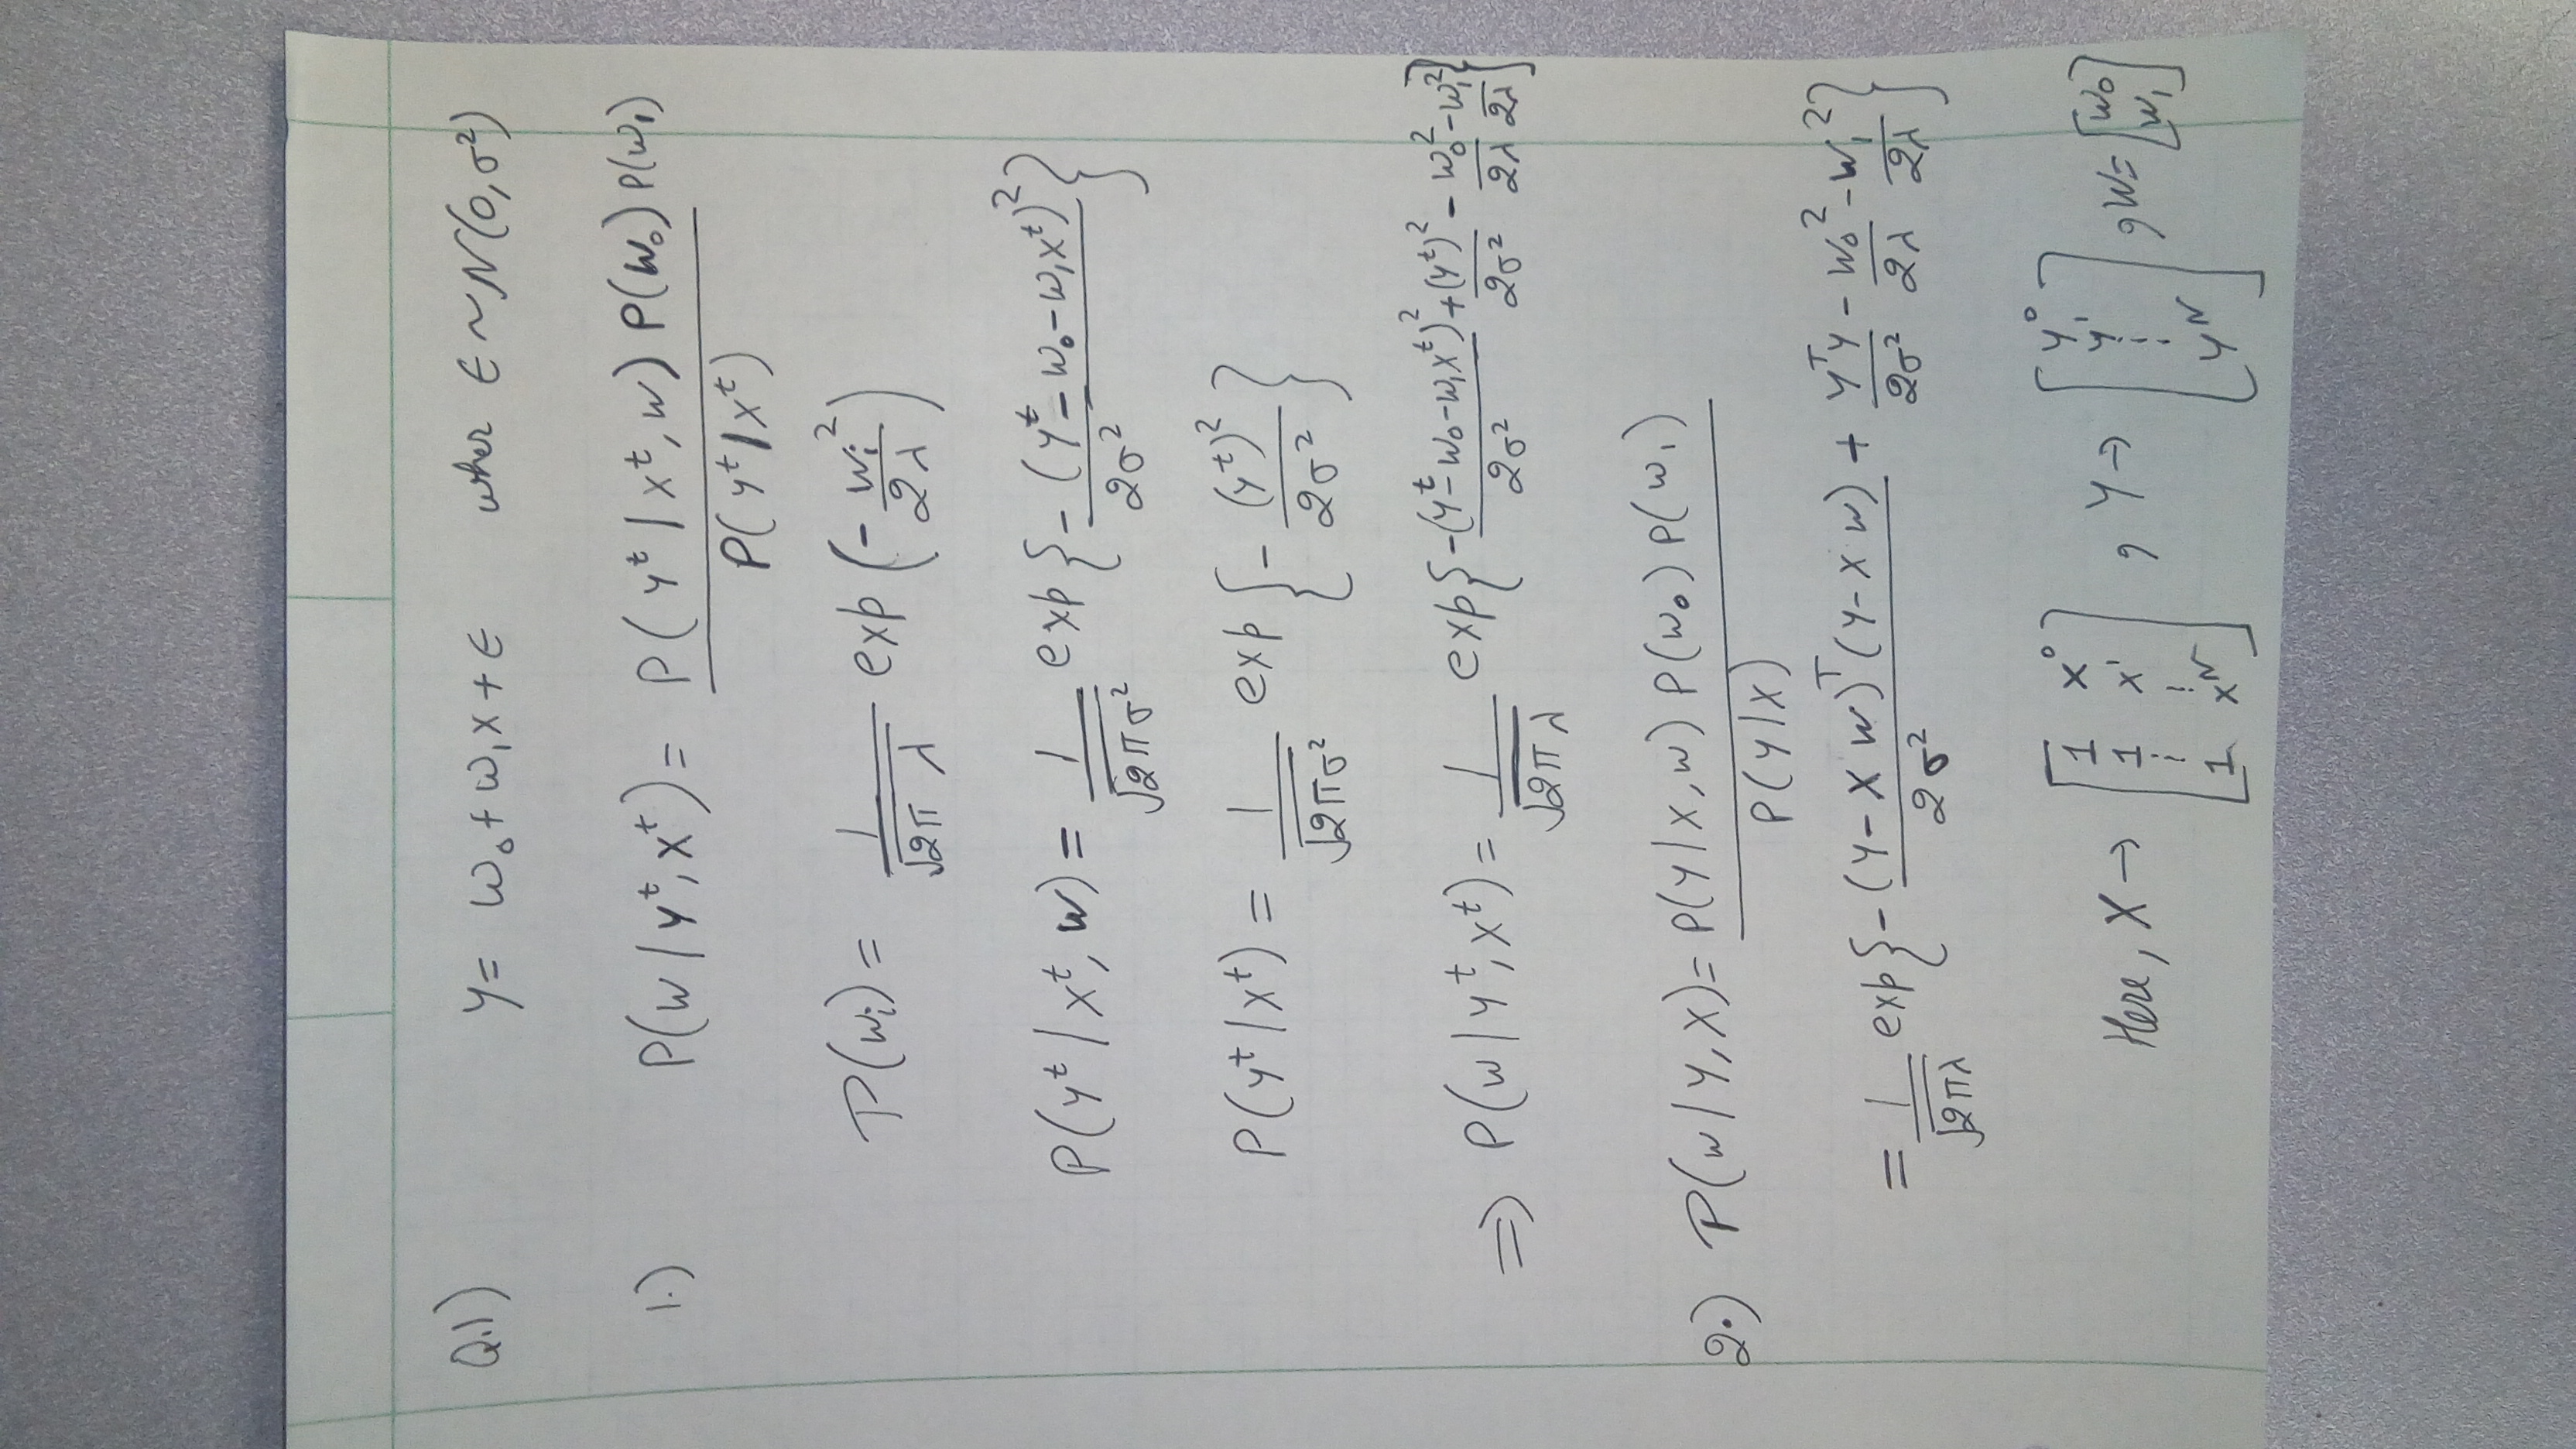
\includegraphics[width=1.4\textwidth, angle=270]{hw9_q1_1.jpg}
		\end{figure}
		\begin{figure}
			\centering
			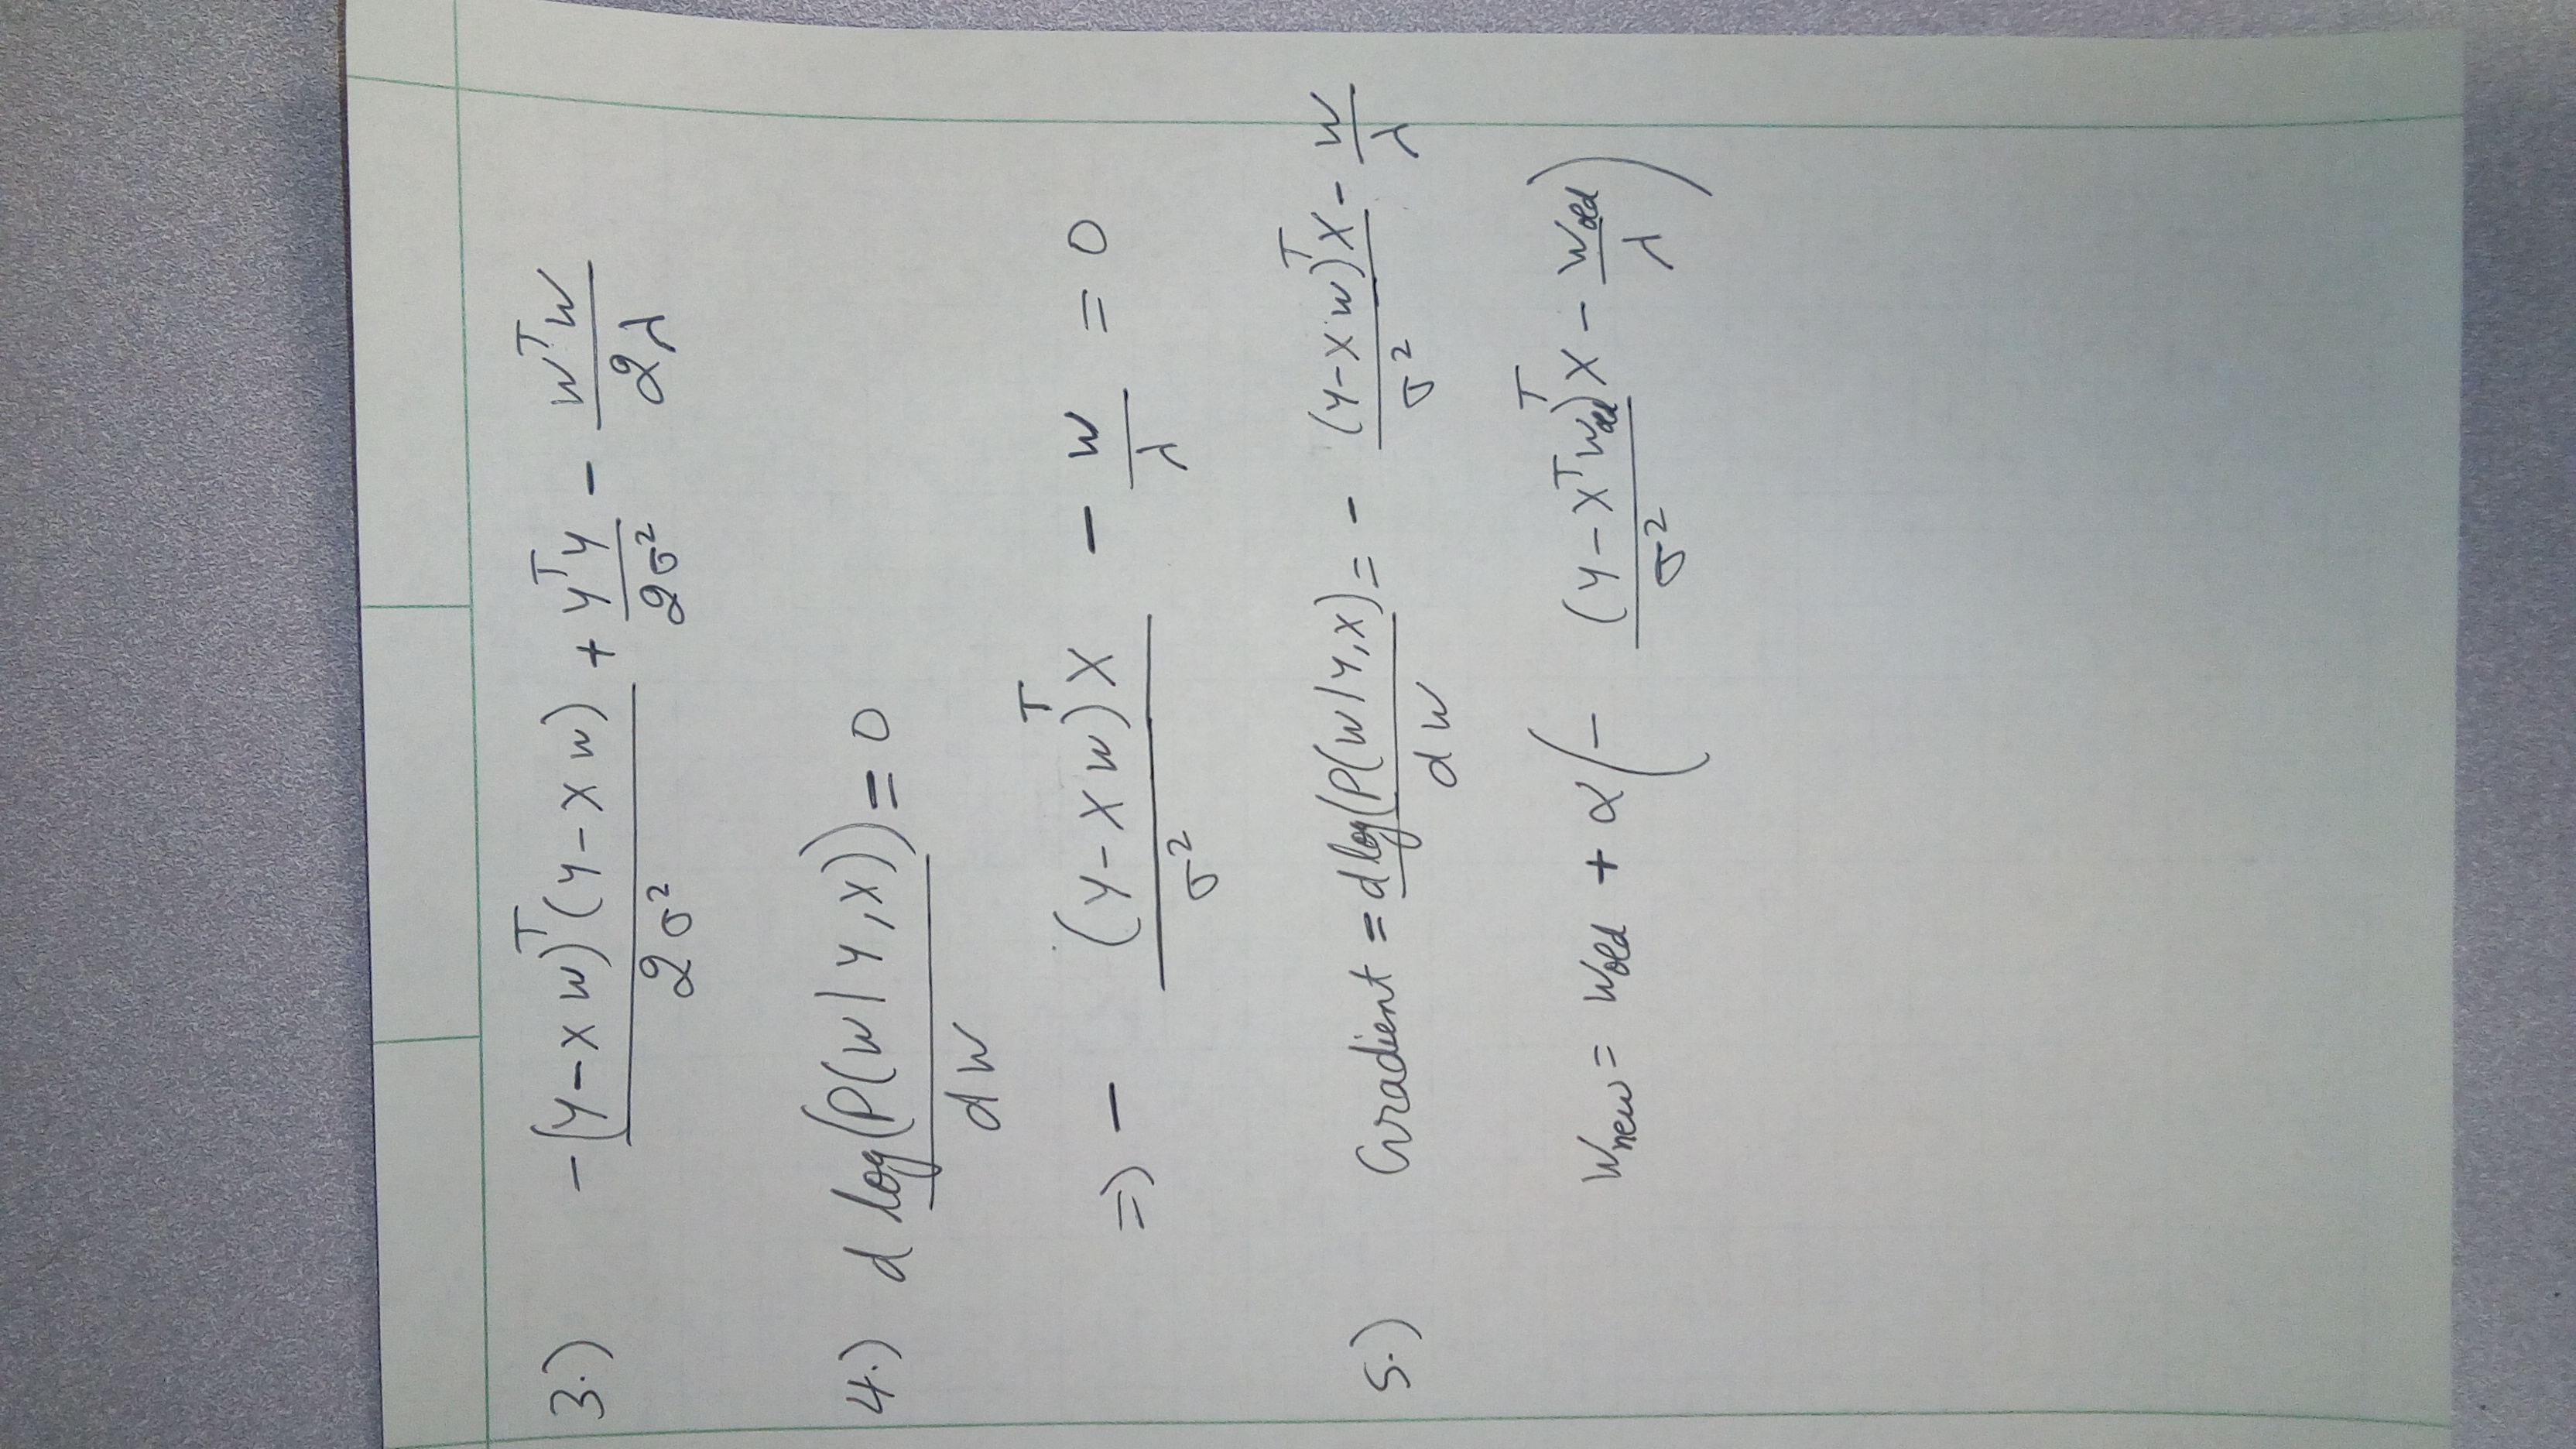
\includegraphics[width=1.4\textwidth, angle=270]{hw9_q1_2.jpg}
		\end{figure}
		\begin{figure}
			\centering
			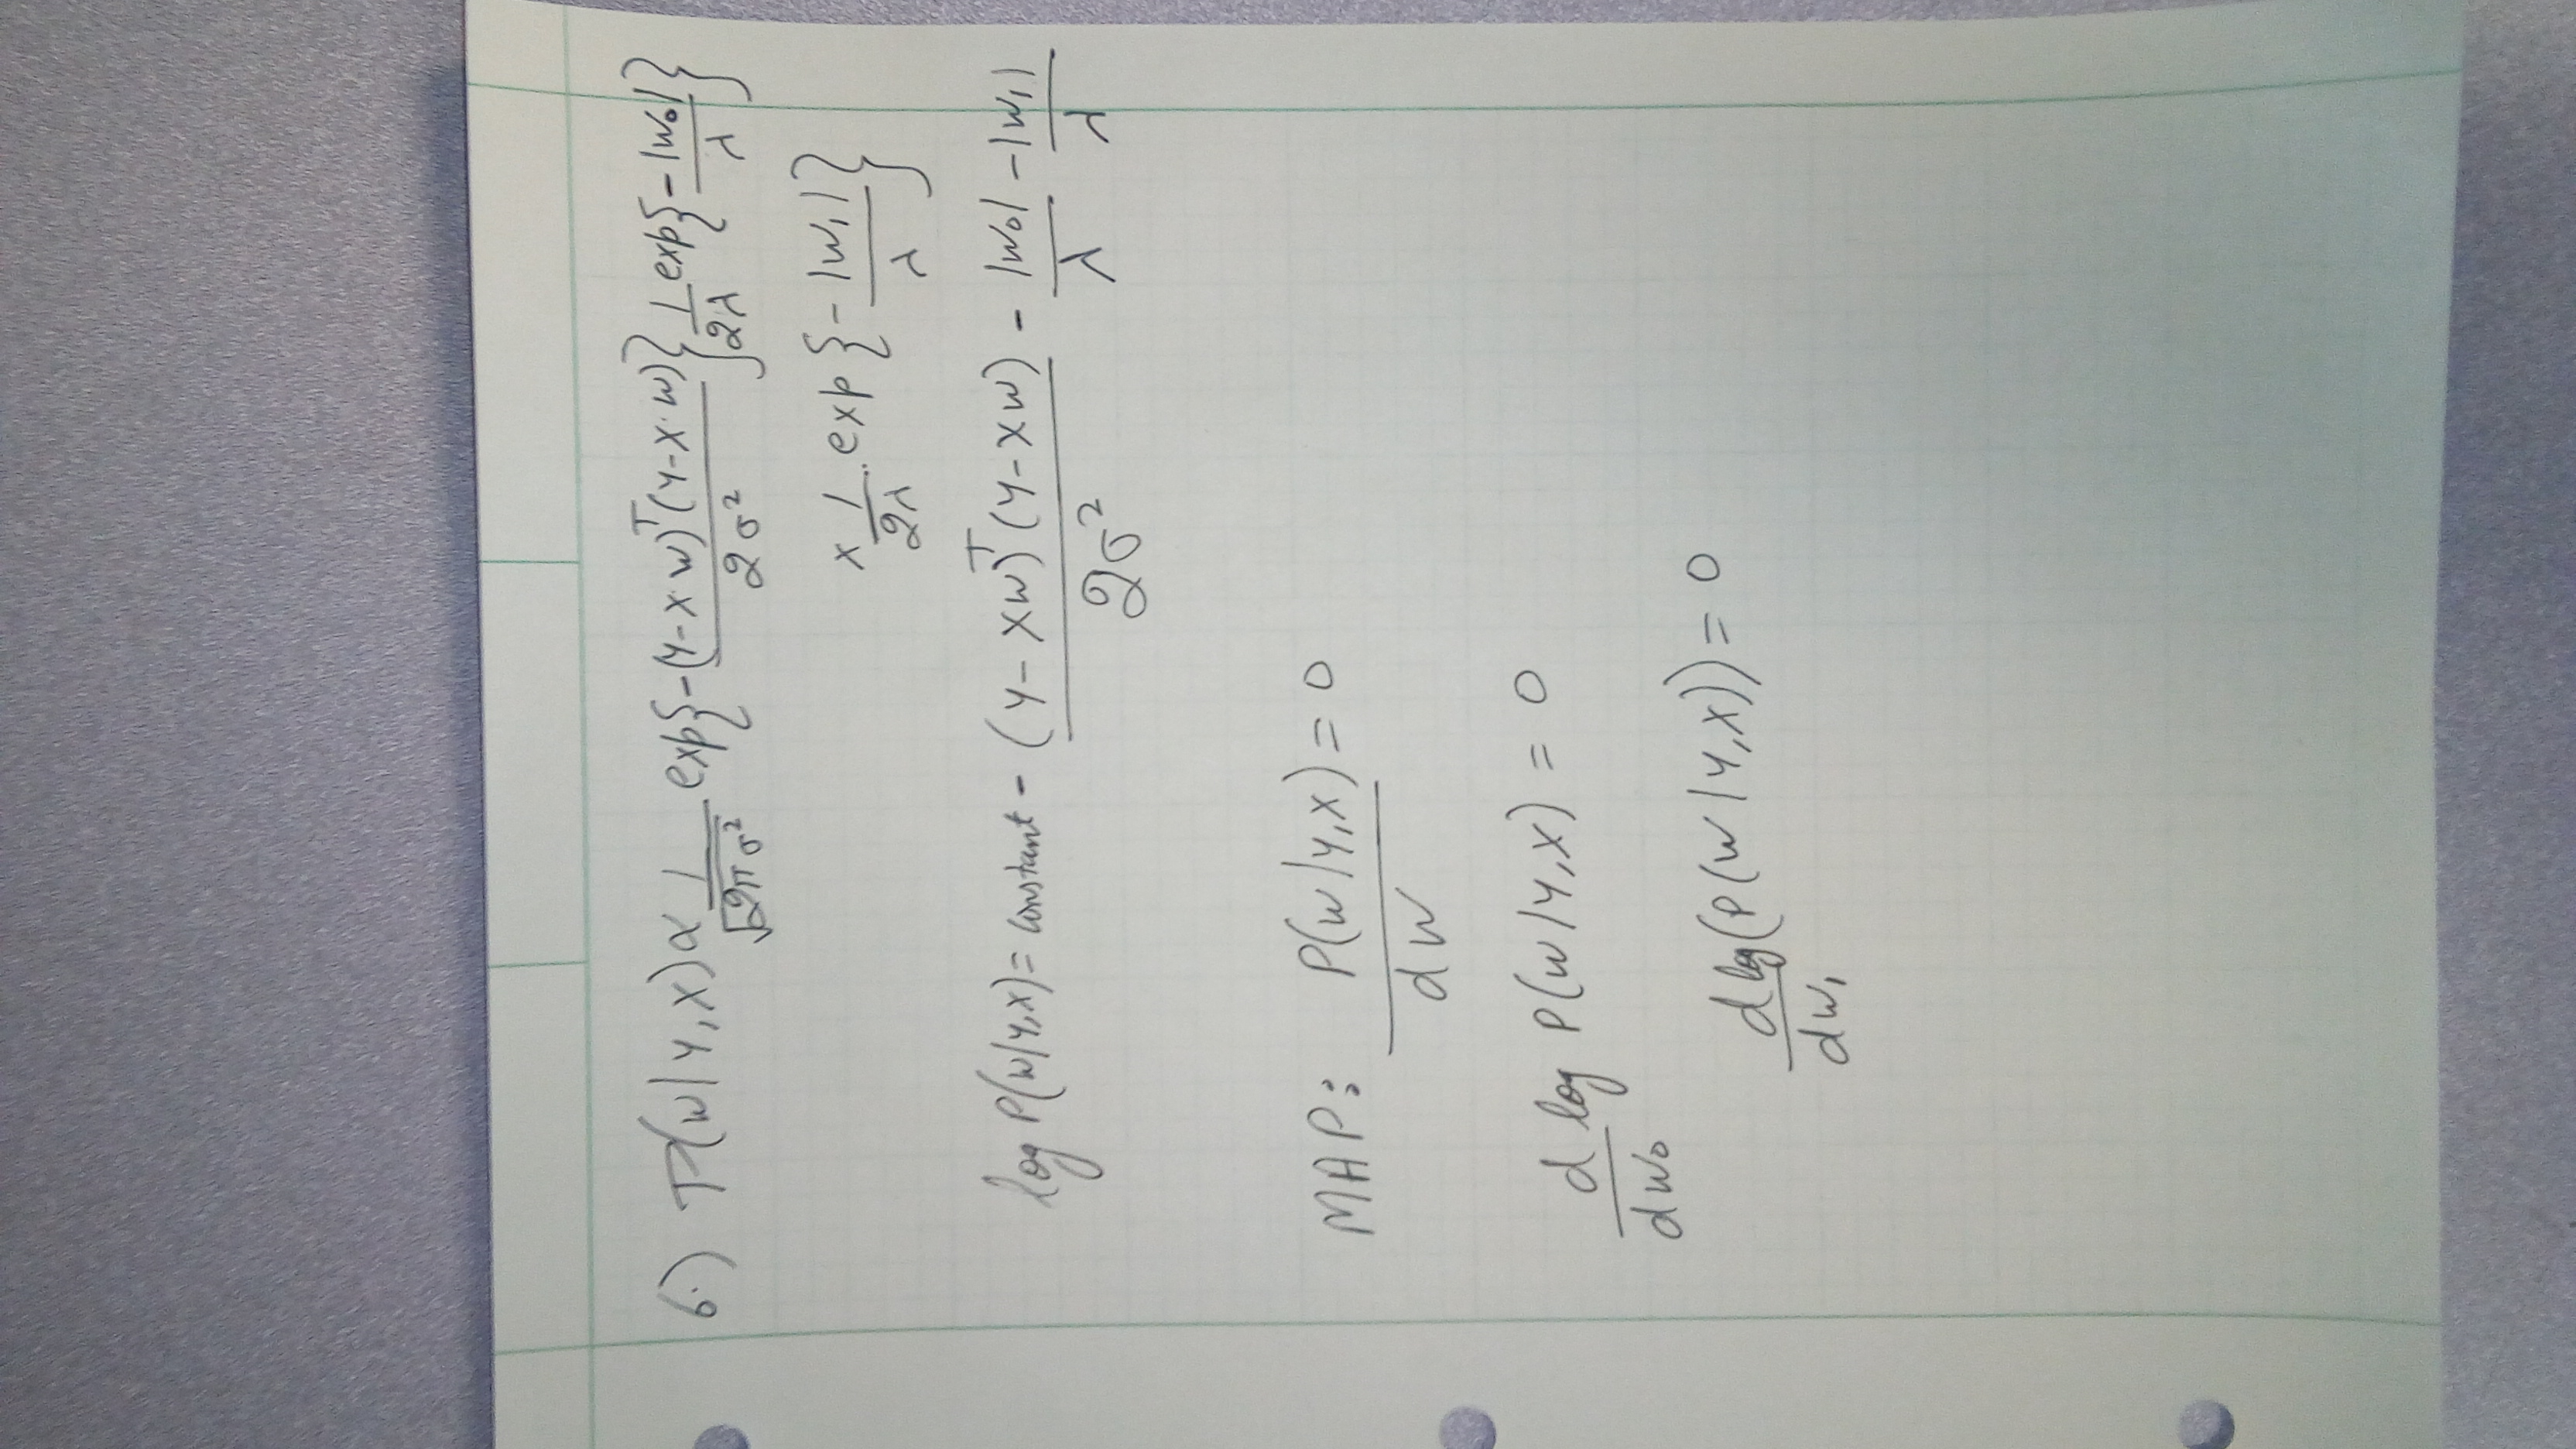
\includegraphics[width=1.4\textwidth, angle=270]{hw9_q1_3.jpg}
		\end{figure}
		
	\end{adjustwidth}
	
	\section{}
	\begin{adjustwidth}{4em}{0pt}
		\subsection{True}
		\subsection{False}
		\subsection{True}
		\subsection{A}
		\subsection{A, C}
		\subsection{Kernel SVM will be lower training error and lower test error. This is because we can choose kernels corresponding to transformations that best describe our model. This is given the Neural network in this question. If we start increasing layers in neural network and we can allow more non-linearities and hence can get better results with neural networks}
	\end{adjustwidth}
	
	\section{}
	\begin{adjustwidth}{4em}{0pt}
		\subsection{}
		\begin{adjustwidth}{4em}{0pt}
			$x_1^2 + x_2^2$
		\end{adjustwidth}
		\subsection{images on new page. Sorry for formatting}
		\begin{figure}
			\centering
			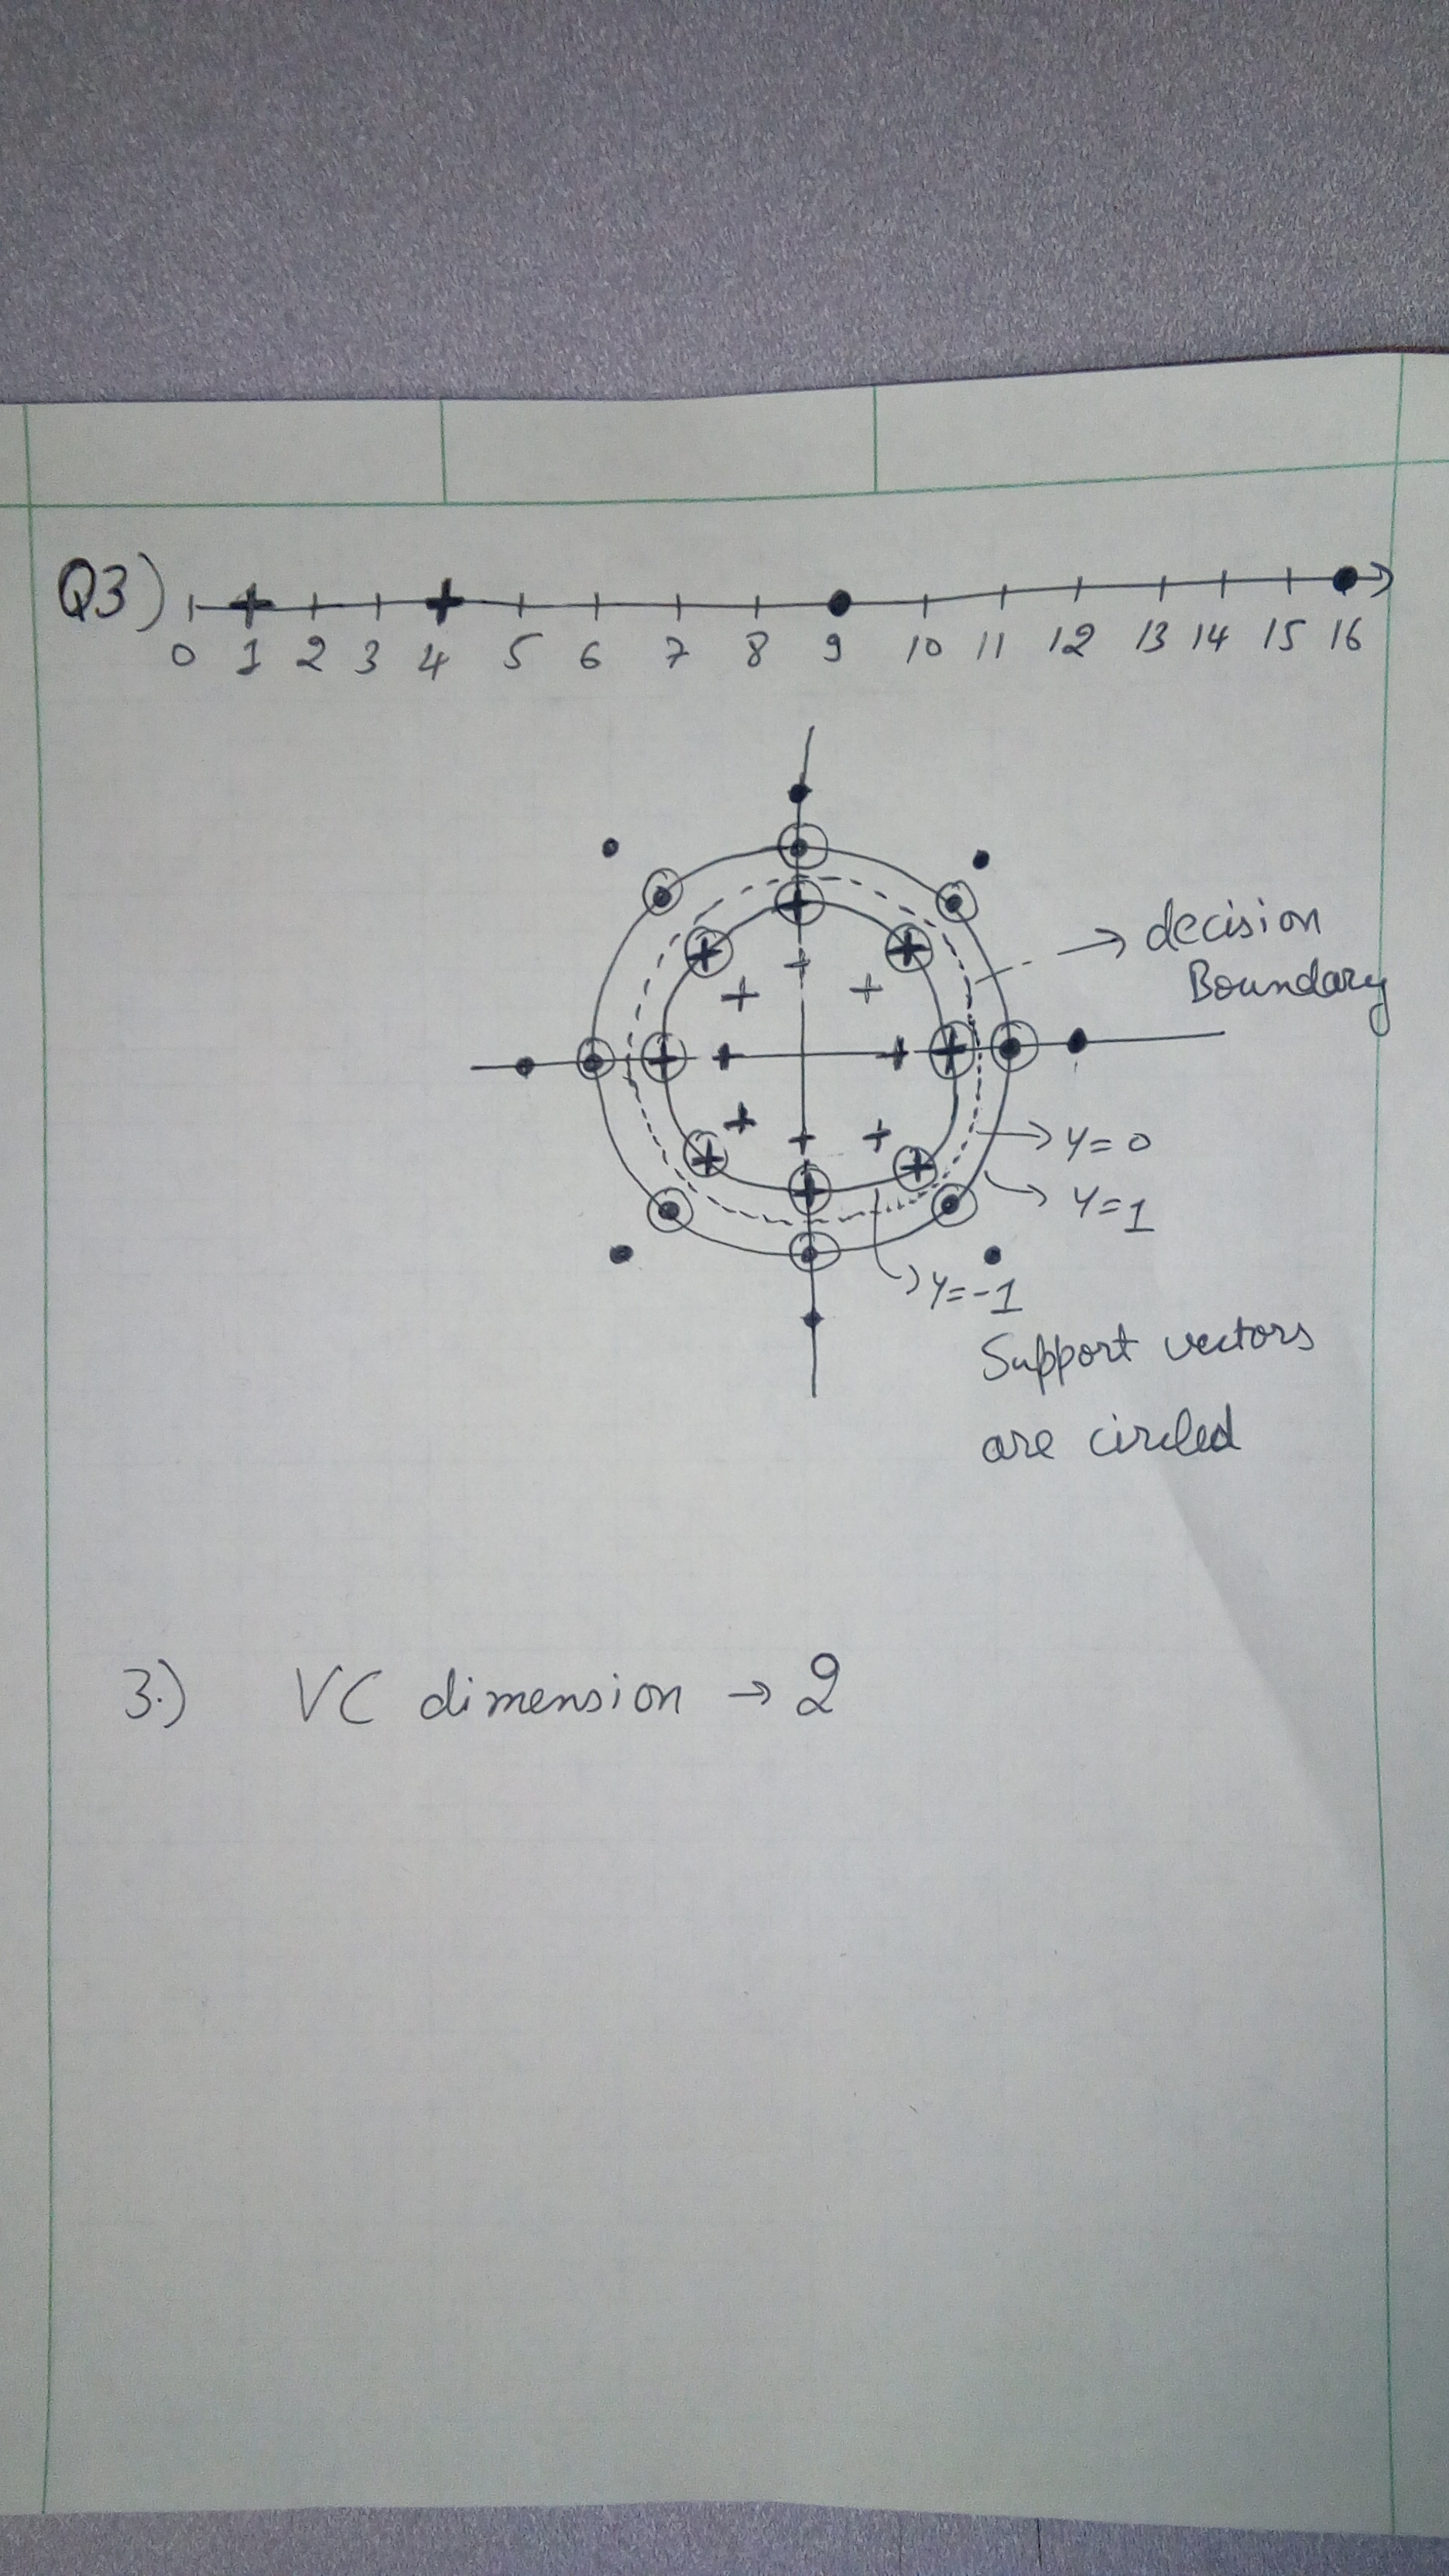
\includegraphics[width=1\textwidth, angle=0]{hw9_q3.jpg}
		\end{figure}
	\end{adjustwidth}
	
	\section{}
	\begin{adjustwidth}{4em}{0pt}
		\subsection{}
		\begin{adjustwidth}{4em}{0pt}
			The appropriate loss function is Hinge loss as it provides tight (convex) upper bound on 0-1 loss function. While this function is convex and continuous, it is not differentiable at 1 but this can be solved using subgradient descent methods.
		\end{adjustwidth}
		\subsection{}
		\begin{adjustwidth}{4em}{0pt}
			Mean squared error loss is appropriate as it square, absolute, continuous and differential function which will help us use techniques like gradient descent or stochastic gradient descent. This function will represent the actual cost of wrong predictions.
		\end{adjustwidth}
		\subsection{}
		\begin{adjustwidth}{4em}{0pt}
			(a) SVM with no kernel (Soft margin): This will allow the error in classification but we will still not be able to classify 100\% samples correctly.\\
			(b) SVM with quadratic kernel with penalty on slack variable C=0: The quadratic kernel will be able to classify each sample correctly as we can see that it is possible to draw an ellipse that divides the two samples. C does not matter as there are no green sample that is surrounded by red and vice versa.\\
			(c) SVM with quadratic kernel with penalty on slack variable C=$\infty$:  The quadratic kernel will be able to classify each sample correctly as we can see that it is possible to draw an ellipse that divides the two samples. C does not matter as there are no green sample that is surrounded by red and vice versa. \\
			(d) Logistic regression (No kernel): Logistic regression with no kernel with have linear surface as separator which will not be able to classify all samples correctly.
		\end{adjustwidth}
	\end{adjustwidth}
	
	\section{Collaboration Policy}
	\subsection{No}
	\subsection{No}
	\subsection{No}
	
\end{document}